\documentclass{article}
\usepackage{graphicx} % Required for inserting images
\graphicspath{{../images/}}

\title{Florida Temperature}
\author{Sam Smith}
\date{October 2023}

\begin{document}

\maketitle

\section{Introduction}

The Correlation Coefficient between years and temperature in Florida from 1901 to 2000 is \textbf{0.53}.
However, temperature data in successive time points are not independent as previous temperatures affect present temperatures. Therefore permutation analysis is necessary to generate a distribution of random coefficients to evaluate the probability that the \textbf{0.53} coefficient happened by chance. I generated 10000 different random permutations of the temperature data and computed their respective correlation coefficient with respect to years. These coefficients were stored a vector. A histogram illustrating the distribution of these coefficients is shown in \textbf{fig 1}.\\

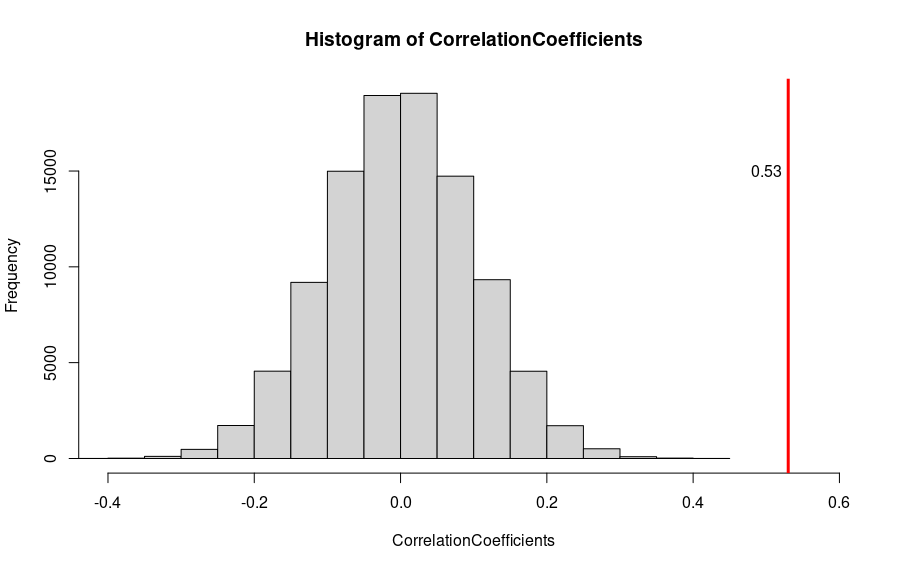
\includegraphics[scale=0.4]{Hist.png}\\
It is clear from \textbf{fig 1} that the correlation coefficients of the 10000 randomly generated temperature values are normally distributed around 0 with a range of -0.340 to 0.397. It is clear from this range and the red line on fig 1 that the real correlation coefficient significantly differs from the correlation coefficients from the permutation analysis.Finally, the percentage of permuated correlation coefficients that exceeded the true corelation value was 0. Therefore it can be said for certain that there is a correlation.
\end{document}
